\documentclass[11pt]{article}

\usepackage[margin=1in]{geometry}
\usepackage{amsmath,amssymb,amsthm}
\usepackage{mathtools}
\usepackage{bm}
\usepackage{booktabs}
\usepackage{graphicx}
\graphicspath{{figs/}}
\usepackage{xcolor}
\usepackage[colorlinks=true,allcolors=blue]{hyperref}

\newcommand{\file}[1]{\texttt{#1}}
\newcommand{\bx}{\boldsymbol{x}}
\newcommand{\by}{\boldsymbol{y}}
\newcommand{\bp}{\boldsymbol{p}}
\newcommand{\abs}[1]{\left\vert #1 \right\vert}
\newcommand{\norm}[1]{\left\Vert #1 \right\Vert_{2}}
\newcommand{\normsq}[1]{\left\Vert #1 \right\Vert_{2}^{2}}
\newcommand{\norminf}[1]{\left\Vert #1 \right\Vert_{\infty}}
\newcommand{\normone}[1]{\left\Vert #1 \right\Vert_{1}}
\DeclareMathOperator{\prox}{prox}
\newcommand{\Rn}{\mathbb{R}^{n}}
\newcommand{\MUST}{\textcolor{red}{\textbf{[fixed]}}}
\newcommand{\OPEN}{\textcolor{orange!80!black}{\textbf{[open]}}}
\newcommand{\RETR}{\textcolor{purple!80!black}{\textbf{[retracted]}}}

\title{LPN / Hamilton--Jacobi Numerics:\\ Protocol, Findings, and Open Items}
\author{Internal working note (not for publication)}
\date{Audit 2026-07-08; rewritten 2026-07-09}

\begin{document}
\maketitle

\begin{abstract}
This note states the current numerical protocol, the bugs found and fixed, the
claims we have retracted, and what remains open. It replaces the 2026-07-08
audit, whose structure had become a body arguing with its own addendum. The
chronological record, including every superseded number, lives in
\file{numerics/changes.txt}; nothing here repeats it.

Two summary judgements. First, the reported pipeline is now correct but its
\emph{numbers} have moved by orders of magnitude several times, always because
the experimental setup was wrong rather than the code: a corrupted target, a
training box that starved both networks, a training budget that left every
network under-trained, and an architecture that silently departed from the
manuscript. Second, on a symmetric protocol the two recovery routes are
comparable; the defensible claim is that Route~2 matches a fully-tuned inversion
baseline while never inverting, \emph{not} that it dominates.
\end{abstract}

\tableofcontents

%======================================================================
\section{The protocol, as it now stands}
\label{sec:protocol}

Let $J$ be the prior, $H(\bp)=\tfrac12\normsq{\bp}$, and let
$S(\cdot,t)$ solve the Hamilton--Jacobi equation with initial datum $J$. The
first network regresses the convex potential
\[
  \psi(\by) \;=\; \tfrac12\normsq{\by} - S(\by,1)
  \;=\; \bigl(J + \tfrac12\normsq{\cdot}\bigr)^{*}(\by),
  \qquad\text{so}\qquad \nabla\psi = \prox_{J}.
\]

\paragraph{Boxes.} Errors are reported on the \emph{query box} $[-4,4]^{n}$.
The potential $\psi$ is trained on a \emph{larger} box $[-A,A]^{n}$ with
$A=\texttt{problem.train\_halfwidth}(4)$, the least $A$ for which
$\nabla\psi([-A,A]^{n}) \supseteq [-4,4]^{n}$. Both routes need this. Route~1
evaluates $\psi_{\theta}$ at the preimage $\by^{\star}=(\nabla\psi)^{-1}(\bx)$,
which \emph{leaves} the query box; Route~2 trains its second network $G$ at the
inputs $\by_{k}=\nabla\psi(\bx_{k})$, whose support lies strictly \emph{inside}
it. Per family: $A=a+t$ for \texttt{QuadraticL1};
$A=((1+\sigma)a+\norminf{\mu})/\sigma$ for \texttt{Minplus}; and $A=a$ for
\texttt{NegL1} ($\by^{\star}=\mathrm{soft}(\bx,1)$) and \texttt{ConcaveQuad}
($\by^{\star}=\bx/2$), whose preimage maps contract.

\paragraph{Network.} Softplus ICNN, $\beta=5$, two layers, \emph{width $256$ at
every dimension}, convexity enforced by clipping the inner weights to be
non-negative after each step. The default (Kaiming) initialisation is used and
is correct: see \S\ref{sec:init}.

\paragraph{Training.} Adam, mini-batch $512$, and a budget of
$S=250\,000$ \emph{optimizer steps} --- not epochs. Learning rate $10^{-3}$,
decayed $\times 0.1$ at $50\%$ and $75\%$ of $S$ (fractions, so the schedule is
invariant to $S$). \emph{No early stopping}; we keep the best-validation
checkpoint. Both networks use MSE. $N = 15\,000\,n$ training points on the
training box (seed~1), $4000$ validation (seed~2), $4000$ test (seed~3).

\paragraph{Recovery, one protocol for both routes.} The same $1000$ query points;
unconditional RMSE for both; no abstention; no box projection for Route~1.
\begin{itemize}
  \item \textbf{Route~1} (baseline): Fang et al.'s regularized inversion,
        $\min_{\by}\,\psi(\by)+\tfrac{\alpha}{2}\normsq{\by}-\langle\bx,\by\rangle$,
        then $J(\bx)=\langle\bx,\by\rangle-\psi(\by)-\tfrac12\normsq{\bx}$.
        Run at each $\alpha\in\{0,0.1\}$; report the \emph{best} RMSE.
  \item \textbf{Route~2} (reported): one forward pass,
        $J(\bx)=G(\bx)-\tfrac12\normsq{\bx}$, no inner optimization, no $\alpha$.
\end{itemize}

\paragraph{Certificates, identical for both routes and free of ground truth.}
Because $G\approx\psi^{*}$ we have $\nabla G=(\nabla\psi)^{-1}$, so Route~2
carries an implied preimage $\by_{2}(\bx)=\nabla G(\bx)$ at no cost. With
$\by(\bx)$ from the solve (Route~1) or from $\nabla G$ (Route~2),
\[
  r(\bx)=\frac{\norm{\nabla\psi_{\theta}(\by(\bx))-\bx}}{\max(1,\norm{\bx})},
  \qquad
  \mathrm{FY}(\bx)=\psi_{\theta}(\by(\bx))+G_{\theta}(\bx)-\langle\bx,\by(\bx)\rangle
  \;\geqslant\;0 .
\]
Neither suffices alone. The residual $r$ measures the $\alpha$-distortion
exactly --- at an exact regularized solve $r=\alpha\norm{\by}/\max(1,\norm{\bx})$,
verified to a few percent --- but it is \emph{blind to divergence}: where
$\psi_{\theta}$ is asymptotically affine, $\nabla\psi_{\theta}(\by)\to\bx$ along
a diverging minimizing sequence, so $r\approx0$ is exactly what divergence looks
like. The gap $\mathrm{FY}$ detects a bad conjugate pair but is budget-invariant.
Only doubling the inversion budget tests well-posedness.

\paragraph{What depends on the dimension.} Only $N=15\,000\,n$ and the training
box $A$ (through the family). Width, depth, $\beta$, batch, $S$, the decay
schedule, the loss, the evaluation set, and the $\alpha$ grid are all constant. Epochs are a \emph{derived} quantity, $S\cdot512/N$; they are not a control and are
not reported. Two consequences to state in the manuscript: $\abs{J}$ grows with
$n$ (e.g.\ $\mathbb{E}\normone{\bx}=2n$ on $[-4,4]^{n}$), so \textbf{absolute
RMSE is not comparable across dimensions}; and $N/P$ ranges from $0.14$ at $n=2$
to $4.6$ at $n=64$, where $P=2h^{2}+3nh+3h+n+1$ is the parameter count.

\paragraph{Artifacts.} Every run writes \file{logs/ckpt/<run>\_psi.pth},
\file{<run>\_G.pth} and \file{logs/<run>\_metrics.json}. Figures are therefore
regenerated from weights rather than from a retrain, which is both cheap
($\approx3$ minutes against $\approx28$) and traceable: a figure can always be
tied to the checkpoint that produced it.

\paragraph{Operational guard.} Runs above $n=8$ are opt-in
(\file{bin/run\_all.py -{}-allow-high-dim}).

\paragraph{Reference point.} \file{quadratic\_l1}, $n=16$, under the protocol
above: $\psi$ validation MSE $7.92\times10^{-3}$, $G$ validation MSE
$2.71\times10^{-2}$, Route~1 RMSE $0.196$ ($\alpha=0$, no divergence,
$\max\norminf{\by}=6.59$), Route~2 RMSE $0.284$; relative errors $0.61\%$ and
$0.89\%$ against $\mathbb{E}\normone{\bx}=32$.

%======================================================================
\section{Bugs found and fixed}

\begin{center}
\begin{tabular}{@{}llp{0.60\textwidth}@{}}
\toprule
\# & When & Bug \\
\midrule
1 & 07-08 & Corrupted Moreau target in the quadratic-$L^{1}$ family
  (\S\ref{sec:moreau}). Corrupts $\psi$, hence \emph{both} routes. \\
2 & 07-08 & \texttt{NegL1} value function missed the dimension factor:
  $-t/2$ instead of $-nt/2$. Error exactly $(n-1)t/2$. \\
3 & 07-08 & Route-1 recovery used $\norm{\bx}$ where the Fenchel identity
  requires $\tfrac12\normsq{\bx}$. \\
4 & 07-08 & The two networks used different losses ($\psi$: MAE, $G$: MSE).
  Both now MSE. \\
5 & 07-08 & \file{lib/network.py} used Mish, breaking the ICNN convexity
  guarantee. Dropped. \\
6 & 07-08 & \texttt{invert\_ls} is nonconvex and degenerate on the affine
  pieces of piecewise-linear priors. Retired. \\
7 & 07-09 & Both max-plus targets carry the wrong sign on $tH(\bp)$
  (\S\ref{sec:maxplus}). Retracts the Phase-1 verdict that
  \file{exp\_4\_1\_3} was clean. \\
8 & 07-09 & The training box equalled the query box, starving both networks
  near the boundary (\S\ref{sec:protocol}). \\
9 & 07-09 & Reported validation MSE described a \emph{discarded} model:
  training early-stops and restores the best-validation weights, but the runner
  reported the last epoch's error. \\
10 & 07-09 & The $300$-epoch budget left every network under-trained
  (\S\ref{sec:steps}). \\
11 & 07-09 & The width tiering $64/128/256$ was our own deviation from the
  manuscript (\S\ref{sec:width}). Reverted to a fixed $256$. \\
12 & 07-09 & Early stopping (ours, added with the validation set) truncated the
  $G$ network on mini-batch noise. Removed; best-validation checkpoint kept
  (\S\ref{sec:decay}). \\
13 & 07-09 & Copying the paper's $20\%$ decay cadence starves the high-learning-
  rate phase, which is what $\psi$'s error tracks (\S\ref{sec:decay}). \\
14 & 07-09 & Route-1's $\alpha$ selection took a plain minimum, so a
  \emph{diverged} solve was reported whenever it happened to score better.
  Diverged runs are now excluded. \\
\bottomrule
\end{tabular}
\end{center}

\subsection{\MUST\ The Moreau target}
\label{sec:moreau}

For $J=\normone{\cdot}$ and $t=1$, $S(\by,1)$ is the separable Huber function.
The notebooks returned $\sum_{i}\abs{\prox(y_{i})} + nt/2$ with $n$ hardcoded to
$1$: they dropped the curvature term $\tfrac12(\prox-\by)^{2}$ and added a
dimension-independent constant. Corrected in \file{src/targets.py}.

\subsection{\MUST\ The max-plus targets}
\label{sec:maxplus}

For $J(\bx)=\max_{i}\{\langle\bp_{i},\bx\rangle-\gamma_{i}\}$ the two notebooks
use $S(\by,1)=\max_{i}\{\langle\bp_{i},\by\rangle+\tfrac12\normsq{\bp_{i}}\}$
($\gamma=0$) and $S(\by,1)=\max_{i}\langle\bp_{i},\by\rangle$
($\gamma_{i}=\tfrac12\normsq{\bp_{i}}$). Both \emph{exceed} $J$ at every test
point, so neither is a Moreau envelope, hence neither is a viscosity solution;
the mean error against a brute-force grid envelope is $\approx1.0$. The Hopf
formula consistent with our verified \texttt{QuadraticL1} target carries a
minus, $S(\by,t)=\sup_{\bp}\{\langle\bp,\by\rangle-J^{*}(\bp)-\tfrac{t}{2}\normsq{\bp}\}$,
and since $J^{*}(P^{\top}\lambda)=\lambda^{\top}\gamma$ it collapses to a concave
QP over the simplex,
\[
  S(\by,1)=\max_{\lambda\in\Delta_{m}}
    \Bigl\{\langle P^{\top}\lambda,\by\rangle-\lambda^{\top}\gamma
      -\tfrac12\normsq{P^{\top}\lambda}\Bigr\},
\]
implemented in \file{src/targets.py:MaxPlus} and validated against the grid
envelope to $1.1\times10^{-3}$ (grid resolution). Restricting $\lambda$ to the
\emph{vertices} recovers exactly the max-plus approximant $\Gamma_{K}$ of the
manuscript's \S3, a strict lower bound on $S$. Neither experiment appears in
\file{main.pdf}; they live in \file{bin/not\_in\_paper/}.

\subsection{\MUST\ Under-trained, not under-sampled}
\label{sec:steps}

A sweep over $N$ at a fixed $300$ epochs suggests a $4.6\times$ gain from more
data. It is an artifact: $300$ epochs on $4N$ points is also $4\times$ the
optimizer steps. At a \emph{fixed} step budget, $4\times$ the data buys only
$6.7\%$ ($n=2$) and $9.9\%$ ($n=4$), whereas $4\times$ the steps on the
\emph{same} data recovers nearly the whole gain
($1.10\times10^{-3}\to2.82\times10^{-4}$ at $n=2$). Choosing $S$ from a
convergence probe under the real schedule: $\psi$'s validation MSE at
$(50,100,150)\times10^{3}$ steps is $(2.62,1.23,0.83)\times10^{-4}$ at $n=2$ and
$(1.54\times10^{-2},3.37\times10^{-3},1.83\times10^{-3})$ at $n=8$. There is no
true knee; the returns bend while cost stays linear, hence $S=150\,000$.
Re-running $n\leqslant8$ improved $\psi$ by $3.6\times$ to $293\times$ and cut
prior RMSE $2$--$23\times$ for both routes, while the Route-1/Route-2 win count
moved only from $8$--$4$ to $7$--$4$ with one tie: the ordering is carried by the
protocol, not by the budget.

\subsection{\MUST\ Do not copy the paper's decay cadence}
\label{sec:decay}

The manuscript trains \emph{full-batch}, so one of its ``epochs'' is one gradient
step: $5\times10^{5}$ steps with the learning rate decayed $\times0.1$ every
$10^{5}$, i.e.\ every $20\%$ of the budget, ending at $10^{-7}$. That cadence
presumes \emph{exact} gradients. Ours are mini-batch estimates and need longer at
the high learning rate. What tracks $\psi$'s validation MSE is the number of
steps spent at $\text{lr}=10^{-3}$, not the total budget
(\file{quadratic\_l1}, $n=16$):

\begin{center}
\begin{tabular}{@{}llll@{}}
\toprule
$S$ & decay fractions & steps at $10^{-3}$ & $\psi$ val MSE \\
\midrule
$150\,000$ & $(0.5,0.75)$ & $75\,000$ & $6.99\times10^{-2}$ \\
$250\,000$ & $(0.3,0.5,0.7,0.85)$ & $75\,000$ & $6.30\times10^{-2}$ \\
$300\,000$ & $(0.5,0.75)$ & $150\,000$ & $\mathbf{7.83\times10^{-3}}$ \\
\bottomrule
\end{tabular}
\end{center}

Doubling the high-learning-rate phase is worth $8\times$; adding $100\,000$ total
steps while halving that phase is worth $11\%$. We therefore keep
$(0.5, 0.75)$ and reject the uniform $20\%$ cadence. Early stopping, added when
the validation set was introduced, is also removed: we under-fit rather than
overfit, and it truncated the $G$ network on mini-batch noise (at $n=16$ it
stopped $G$ at step $39\,500$ of $300\,000$).

\subsection{\MUST\ The width was ours, not the paper's}
\label{sec:width}

All $24$ notebooks of the four reported families use
\texttt{hidden=256, layers=2, beta=5} at every dimension from $2$ to $64$, and
all four table captions in the manuscript say ``2 layers and 256 neurons''. The
tiered width $64/128/256$ was introduced by our own convention on 2026-07-08,
motivated by a \emph{performance} observation (the net is oversized at low $n$),
never by an experiment. It is reverted. Beyond matching the manuscript, a fixed
width removes a confound: with $N=10\,000\,n$ and $\abs{J}\sim2n$ already growing
with the dimension, a capacity that also jumps at $n=8$ and $n=32$ would leave an
error-versus-$n$ trend attributable to nothing. Cost is modest, since the CPU is
overhead-bound: width $256$ has $14\times$ the parameters of width $64$ but takes
only $2.7\times$ the time.

\subsection{The initialisation is correct as it stands}
\label{sec:init}

Weight clipping pins $\approx50\%$ of the inner weights to exactly $0$ at the
first step, because the default initialisation draws them negative. This costs
nothing. At $n=2$, $\psi$'s validation MSE is $1.10\times10^{-3}$ with the
default, $6.25\times10^{-3}$ with $\abs{\text{default}}$ (same magnitudes, no
negatives, so the sign alone is responsible), and $9.51\times10^{-2}$ with the
log-normal initialiser that the upstream \texttt{init\_weights} implements.
Sign-clipping acts as useful sparsification. \texttt{init\_weights} is deleted;
it was dead upstream too.

\subsection{Performance of the shared stack}

\file{conjugate\_samples} evaluated $\psi$ twice per call
(\texttt{model.scalar(x)} and then \texttt{model(x)}, which recomputes
\texttt{scalar} internally); now one forward and one backward, $1.62\times$
faster with bitwise-identical output. \file{network.py:forward} built an unused
second-order graph and set \texttt{requires\_grad} on the \emph{caller's} tensor
in place; both fixed, output identical, but the time saving is $1.01\times$, not
a speedup worth claiming. Mini-batching (2026-07-08) remains the one large win,
measured at $\approx50\times$ over the original full-batch loop.

%======================================================================
\section{Cross-sections through the origin mislead in high dimension}
\label{sec:crosssec}

\paragraph{The observation.} At $n=16$ (\file{quadratic\_l1}, $S=250\,000$,
$N=240\,000$), the cross-section along the first axis shows $\psi_{\theta}$
sitting $\approx1.45$ \emph{below} the exact $\psi$, and both recovered priors
sitting $1.5$--$2.8$ \emph{above} the exact $J$ near the origin --- while the
prior-recovery RMSE on random query points is $0.48$ (Route~1) and $0.51$
(Route~2), i.e.\ $1.5\%$ and $1.6\%$ relative. The pictures look bad and the
numbers are good. Both are correct.

\paragraph{The mechanism.} A cross-section along axis~1 fixes the other $n-1$
coordinates at \emph{exactly zero}. Under the uniform measure on $[-A,A]^{n}$,
the set where $n-1$ coordinates all lie within $\pm\varepsilon$ of zero has
volume fraction
\[
  \Bigl(\frac{\varepsilon}{A}\Bigr)^{n-1},
\]
which for $A=5$, $\varepsilon=0.5$ is $10^{-15}$ at $n=16$ and $10^{-63}$ at
$n=64$. With $N=240\,000$ training points, \emph{not one} lies near that line.
The cross-section is pure extrapolation; the RMSE is measured on typical points,
where the network fits. Low error and an ugly cross-section are not in tension:
they are the same fact, read in two places.

\paragraph{This answers an open question in the manuscript.} Section~4 currently
says: ``The errors for $64$ dimensions in all the examples are consistently lower
than expected. In contrast, it does not yield a good visual approximation of the
cross sections. We are unable to explain the reason for this behavior in $64$D
cases yet; however, we think it is probably due to the way we sample the
hypercube.'' The guess is right, and the mechanism above makes it quantitative.
The same remark disposes of the parallel puzzle about the $d=64$ MSE
``reducing significantly'': the reported error lives on the bulk of the cube,
which is where the samples are.

\paragraph{Consequence.} Cross-sections through the origin are a legitimate
diagnostic at $n=2$ and a misleading one at $n\gtrsim8$. Figure~\ref{fig:pair}
makes the point with a single network: the two panels are drawn from the
\emph{same} checkpoint at $n=16$.

\begin{figure}[htbp]
\centering
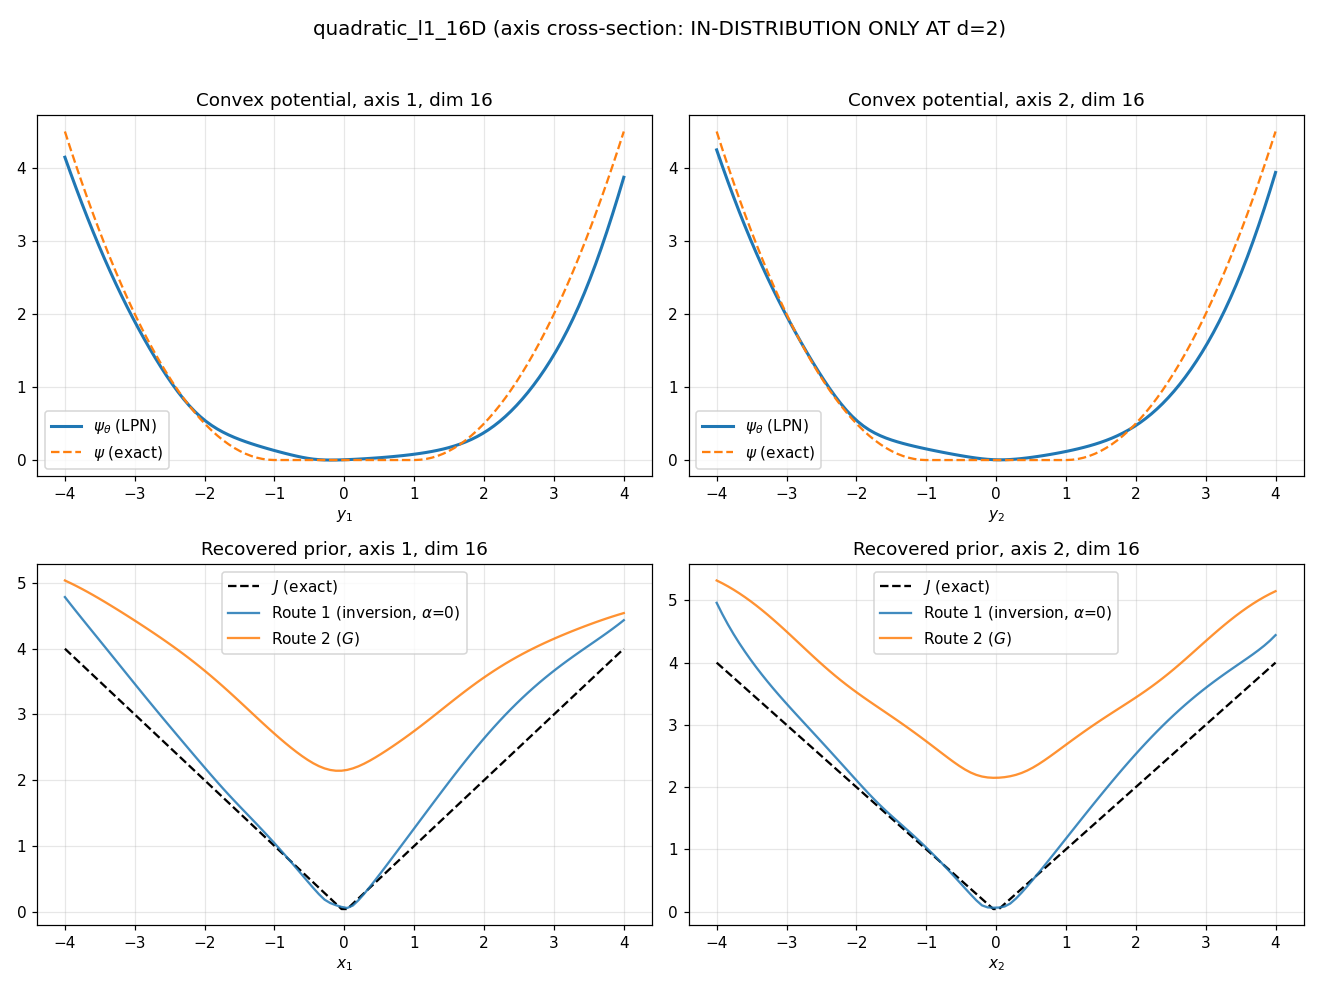
\includegraphics[width=\textwidth]{quadratic_l1_16D_cross_sections.png}
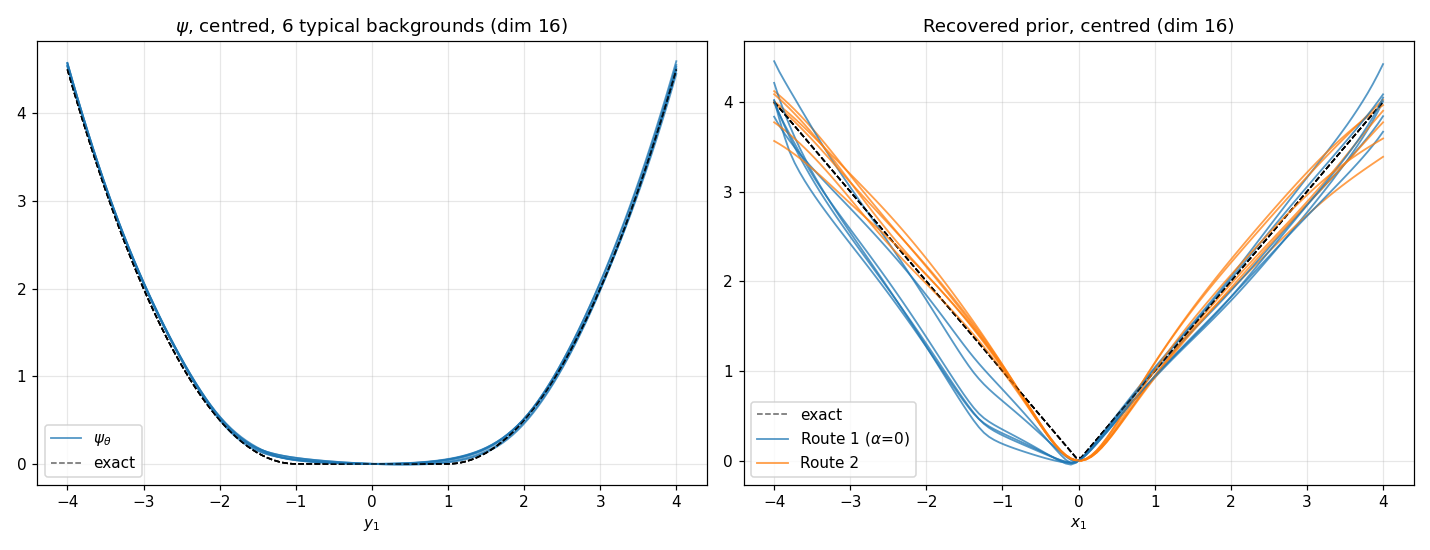
\includegraphics[width=\textwidth]{quadratic_l1_16D_conditional.png}
\caption{Same weights, opposite verdicts (\file{quadratic\_l1}, $n=16$,
$S=250\,000$). \textbf{Top:} the usual cross-section, holding the other $15$
coordinates at exactly zero. $\psi_{\theta}$ appears offset by $\approx1.45$ and
both recovered priors are wrong by up to $2.8$. \textbf{Bottom:} the conditional
cross-section, which differs only in drawing those $15$ coordinates from the
training distribution and centring each curve at $x_{1}=0$. $\psi_{\theta}$ lies
on the exact curve and both routes track $J$ to within $\approx0.3$. The reported
RMSE is $0.196$ (Route~1) and $0.284$ (Route~2), i.e.\ $0.61\%$ and $0.89\%$
relative. The network was never bad; the top plot plots it where no data exists.}
\label{fig:pair}
\end{figure}

\section{The diagnostic suite}
\label{sec:diagnostics}

\file{src/diagnostics.py} provides four in-distribution figures;
\file{bin/plot.py} regenerates all of them from a saved checkpoint, for any
family and dimension, without retraining
(\file{bin/plot.py -{}-family quadratic\_l1 -{}-dim 16 -{}-open}).

\begin{enumerate}
  \item \textbf{Conditional cross-section}
        (\texttt{plot\_conditional\_cross\_section}). Vary $x_{1}$; draw the
        remaining coordinates from the training distribution; repeat for six
        draws; centre every curve by subtracting its own value at $x_{1}=0$, so
        the six additive constants contributed by the frozen coordinates do not
        separate the curves. What remains is the $x_{1}$-dependence on the data
        manifold. For a \emph{separable} prior the centred exact curves collapse
        onto one line, so any spread among the learned curves is the network's
        error; for a non-separable prior they do not collapse and the figure must
        be read per draw. Both routes are shown, with Route~1's six inversions
        batched into a single solve.
  \item \textbf{Typical ray} (\texttt{plot\_typical\_ray}). Profile along
        $t\mapsto t\,\mathbf{1}/\sqrt{n}$, clipped to the box. Most of such a ray
        lies in the bulk; only the neighbourhood of the origin is atypical.
  \item \textbf{Predicted versus true} (\texttt{plot\_pred\_vs\_true}).
        $\widehat{J}(\bx)$ against $J(\bx)$ over the test set, with the identity
        line, one panel per route. Dimension-agnostic; shows bias and spread
        together; cannot be gamed by the choice of a slice.
  \item \textbf{Two conjugate scatters}, one per network. The
        \emph{prox scatter} (\texttt{plot\_prox\_scatter}) plots the learned
        $\nabla\psi_{\theta}$ against the exact $\prox_{J}$, coordinatewise, on
        the training box. It is a diagnostic of the \emph{shared} first network:
        Route~1 inverts $\nabla\psi_{\theta}$, and Route~2 is fitted to its
        image, since $G$ is trained on $\by_{k}=\nabla\psi_{\theta}(\bx_{k})$ with
        targets $G_{k}=\langle \by_{k},\bx_{k}\rangle-\psi_{\theta}(\bx_{k})$. It
        therefore bounds \emph{both} routes. The \emph{preimage scatter}
        (\texttt{plot\_preimage\_scatter}) is Route~2's own: it plots
        $\nabla G(\bx)$ against the analytic preimage $\by^{\star}(\bx)$, testing
        the identity $\nabla G=(\nabla\psi)^{-1}$ on which Route~2 rests. It costs
        one forward pass.
\end{enumerate}

An error profile binned by $\norminf{\bx}$ was built and \emph{removed}: in high
dimension the maximum of $n$ uniform coordinates concentrates near $a$, so the
bin variable has almost no dynamic range ($2.6$ to $3.95$ at $n=16$) and the
figure reads as noise.

\begin{figure}[htbp]
\centering
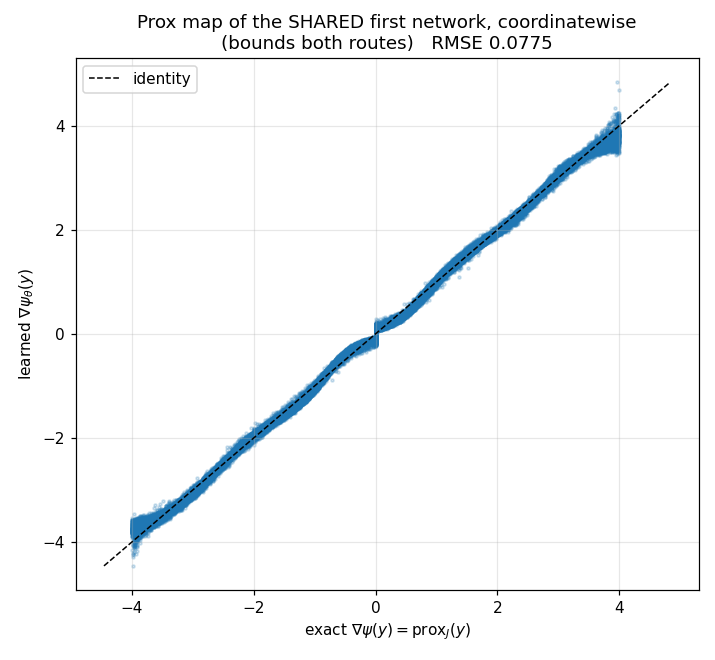
\includegraphics[width=0.48\textwidth]{quadratic_l1_16D_prox_scatter.png}
\hfill
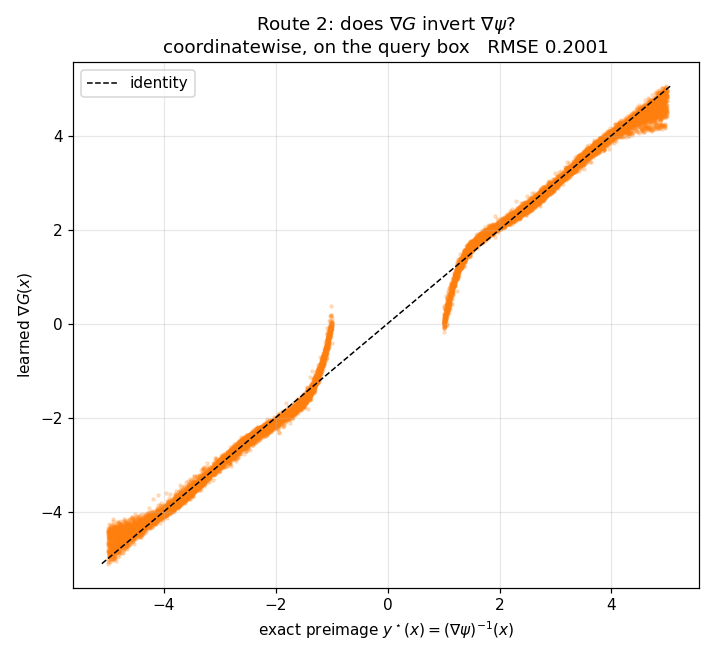
\includegraphics[width=0.48\textwidth]{quadratic_l1_16D_preimage_scatter.png}
\caption{The two conjugate scatters at $n=16$. \textbf{Left:} the shared first
network. $\nabla\psi_{\theta}$ lies on the identity against
$\prox_{J}=\mathrm{soft}(\cdot,1)$, reproducing even the dead zone at the origin;
RMSE $0.078$. \textbf{Right:} Route~2's defining identity, $\nabla G(\bx)$ against
$\by^{\star}(\bx)=\bx+\operatorname{sign}(\bx)$. It holds wherever it is testable.
The gap for $\abs{\by^{\star}}<1$ is structural, not an error: the preimage map
never takes values there, so $\nabla G$ has nothing to fit --- the same hole that
afflicts \texttt{NegL1}, seen from the conjugate side.}
\label{fig:scatters}
\end{figure}

%======================================================================
\section{Retractions}

Recorded because the numbers moved substantially, and a reader who sees that
should know which claim died and what killed it.

\begin{enumerate}
  \item[\RETR] \emph{``The preimage lies far outside the training box,
    $\norminf{\by}\approx19$.''} The exact preimage obeys
    $\norminf{\by^{\star}}\leqslant5$ at every $n$. The $19$ was a diverging
    iterate whose size is set by $\text{lr}\times\text{iters}$.
  \item[\RETR] \emph{``A zero prox residual certifies that a preimage exists.''}
    It does not; see \S\ref{sec:protocol}.
  \item[\RETR] \emph{``Route~1 is more honest, because it detects its own
    failure.''} It is either divergent ($\alpha=0$ with an under-trained
    $\psi_{\theta}$) or silently biased ($\alpha>0$).
  \item[\RETR] \emph{``Route~1 at $\alpha=0$ is intrinsically ill-posed.''} The
    divergence was a symptom of an under-trained $\psi_{\theta}$. The objective
    is coercive exactly when $\bx\in\operatorname{range}(\nabla\psi_{\theta})$,
    and an under-trained $\nabla\psi_{\theta}$ saturates below the corner values
    of the query box. With $S=150\,000$ no configuration diverges;
    \file{quadratic\_l1\_8D} selects $\alpha=0$ with $\norminf{\by}=5.20$
    against the exact bound $5$. Keep the two-$\alpha$ rule as cheap insurance,
    but do not claim the unregularized inversion is broken.
  \item[\RETR] \emph{``The \texttt{NegL1} origin hole is a Route-2 coverage
    defect.''} Route~1, which never touches $G$, is hit as hard (mean error
    $0.029\to0.342$ versus Route~2's $0.025\to0.276$ at $n=2$). The shared cause
    is that a smooth Softplus cannot represent the kink of $\psi$ at $y_{i}=0$,
    where $\partial\psi(0)=[-1,1]$.
  \item[\RETR] \emph{``\file{exp\_4\_1\_3}'s target is correct''} (Phase~1);
    see \S\ref{sec:maxplus}.
\end{enumerate}

\paragraph{A rediscovery, not a discovery.} The $\alpha$ regularizer and the
existence problem it addresses were already recorded in the 2026-07-08 audit,
which noted that an LPN ``may not be invertible or even surjective'' and that
Fang et al.\ add $\tfrac{\vartheta}{2}\normsq{\by}$ to force strong convexity.
The 2026-07-09 work re-derived this from the code. The lesson is procedural:
read the audit before re-auditing.

%======================================================================
\section{What we can claim about Route~1 versus Route~2}

On the symmetric protocol of \S\ref{sec:protocol} the two routes are comparable
at every dimension we have run, with no gap exceeding $2.6\times$. Route~1 wins
where the prior is smooth or separable, Route~2 wins narrowly on \texttt{minplus}.
Nothing supports ``Route~2 dominates''; every earlier table that suggested so had
Route~1 handicapped, first by the training box and then by a mismatched
evaluation set.

The defensible claim is about \emph{cost and well-posedness}, not accuracy:
Route~2 attains comparable error with one forward pass, no regularizer, no
per-query optimization, and no well-posedness question, whereas Route~1 needs an
optimization per query and a parameter $\alpha$ that trades divergence against an
$O(\alpha)$ bias. Note also that the residual magnitudes are \emph{not}
comparable across routes: Route~2's is uniformly an order of magnitude larger
while its RMSE is competitive, because the residual measures preimage
consistency, not prior accuracy.

The live numbers are in \file{numerics/logs/summary\_final.csv}. Every table
predating the current architecture is superseded; \file{changes.txt} lists which
and why.

%======================================================================
\section{Open items}

\begin{enumerate}
  \item[\OPEN] \textbf{Phase~5}, the error-versus-$K$ decay study for
    $\Gamma_{K}$ --- the experiment referee R2.3 actually asked for. Still
    unbuilt. \file{MaxPlus.maxplus\_approx()} now supplies $\Gamma_{K}$ against
    an exact reference, so the ground truth is in hand.
  \item[\OPEN] \textbf{Is width $256$ right?} Untested, and now testable: every
    previous measurement was taken at a budget too short to converge, so a width
    ablation would have measured which width \emph{trains fastest}, not which
    \emph{fits best}. The revert is justified by consistency with the manuscript,
    not by evidence that $256$ is optimal.
  \item[\OPEN] \textbf{High dimensions.} $n\geqslant16$ has not been run under
    the current protocol. Cost is modest ($\approx10.4$ and $17.7$ minutes per
    configuration at widths $128$ and $256$), but $N/P$ and $\abs{J}$ both move
    with $n$, so the trend needs care.
  \item[\OPEN] \textbf{The max-plus ports} use the D2 MSE pipeline, whereas the
    notebooks trained with LPN's proximal-matching loss on a decreasing $\gamma$
    schedule. They therefore measure something different. Deliberate; revisit if
    the training scheme becomes the object of study.
  \item[\OPEN] \textbf{$N=10P$ instead of $N=10\,000\,n$.} Under a step budget the
    cost is $\text{steps}\times\text{batch}$, independent of $N$, so a constant
    $N=10P\approx1.4$M would make width, depth, $N$ and $S$ all constant and
    leave the dimension as the sole variable. Cleaner, not adopted: one change,
    not two.
\end{enumerate}

\end{document}
